% discuss numerical simulation - transfer from L1 to the Moon type orbit
% compare with the transfer using invariant manifolds
\section*{}
\subsection*{Numerical Simulation}
\begin{frame} %-----------------------------------------------%
\frametitle{Transfer example}
\begin{itemize}
	\item Transfer from \( L_1 \) to periodic orbits near Moon
	\item Generate reachable set using computational geometric optimal control over fixed horizon
	\item Compare to transfer via invariant manifolds
\end{itemize}
	\begin{figure} 
	\centering 
	\begin{subfigure}[htbp]{0.5\textwidth} 
		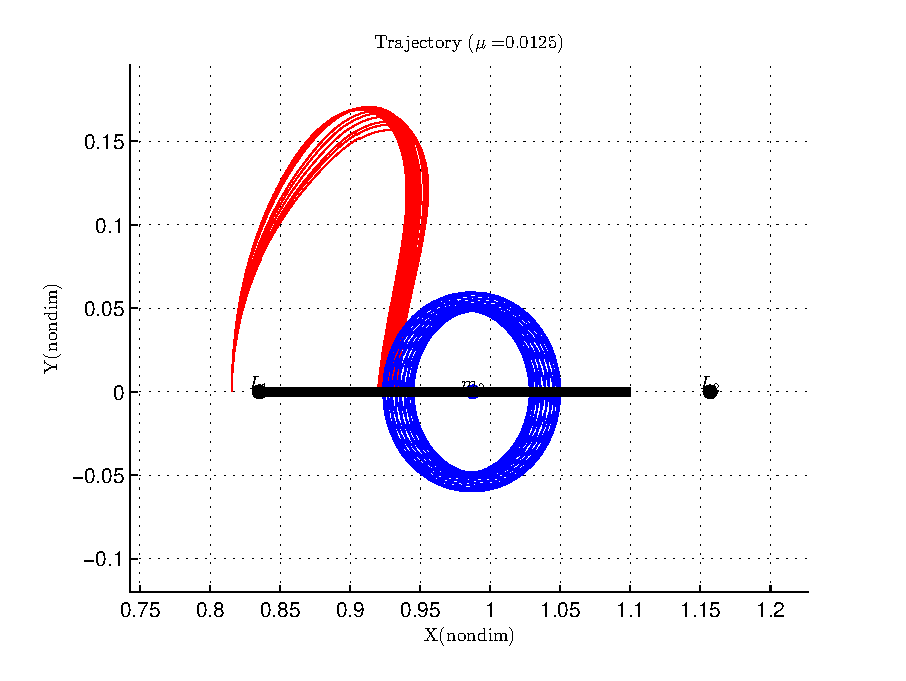
\includegraphics[width=\textwidth]{reach_trajectory}  
	\end{subfigure}~
	\begin{subfigure}[htbp]{0.5\textwidth} 
		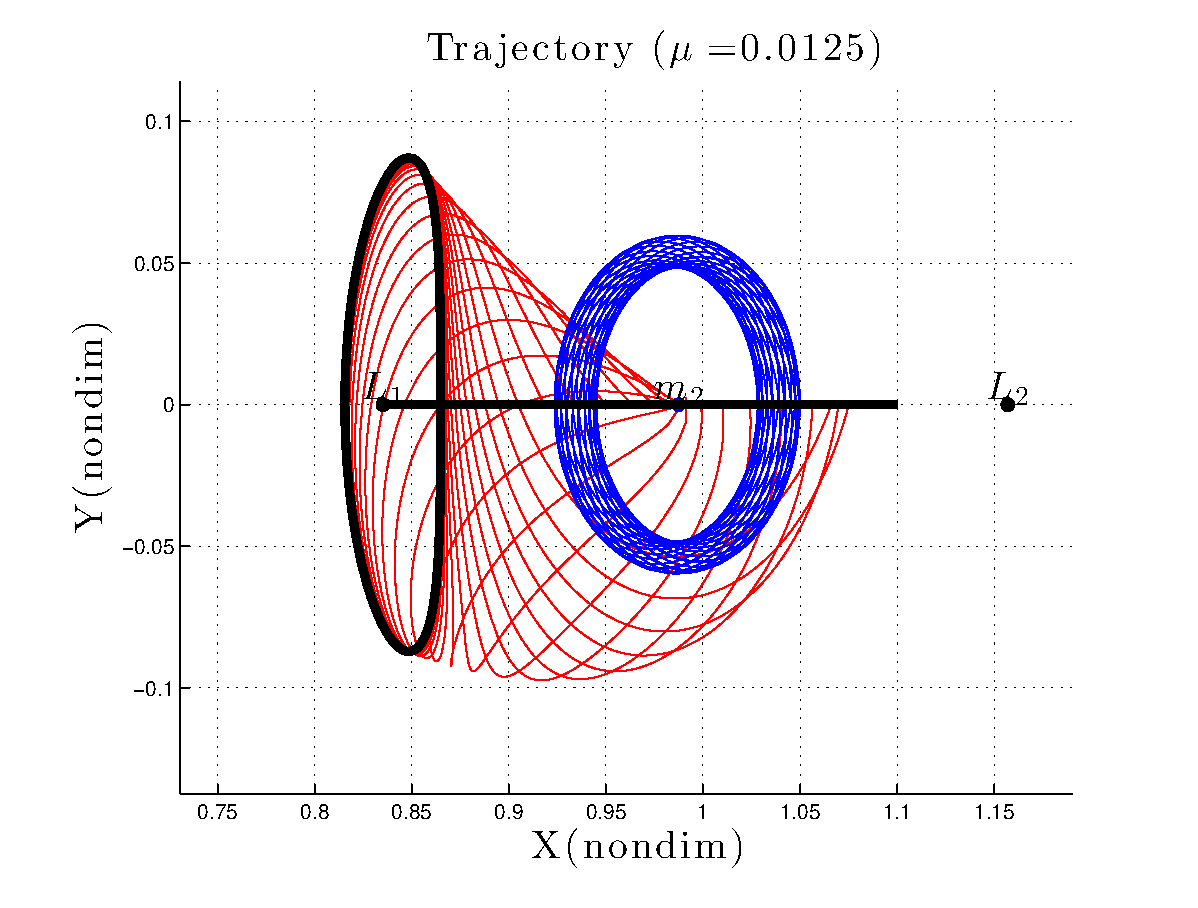
\includegraphics[width=\textwidth]{manifold_trajectory} 
	\end{subfigure} 
	\end{figure}
\end{frame} %------------------------------------------------%

\begin{frame}%------------------------------------------------%
\frametitle{Transfer Example}
\begin{itemize}
	\item Reachability set on Poincar\`e section
	\item Low-thrust propulsion allows for intersection
	\item Portion of unstable manifold does not intersect
	\item Invariant manifold has longer time of flight than reachable set \( t_f \approx 3.1 \) vs. \( t_f \approx 1.4 \)
\end{itemize}
	\begin{figure} 
	\centering 
	\begin{subfigure}[htbp]{0.5\textwidth} 
		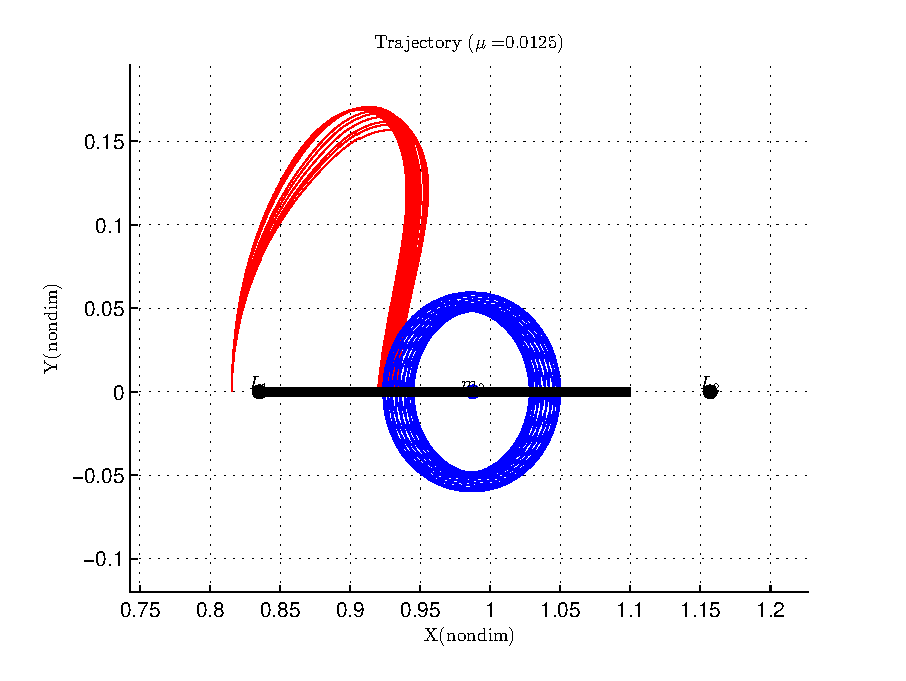
\includegraphics[width=\textwidth]{reach_trajectory}  
	\end{subfigure}~
	\begin{subfigure}[htbp]{0.5\textwidth} 
		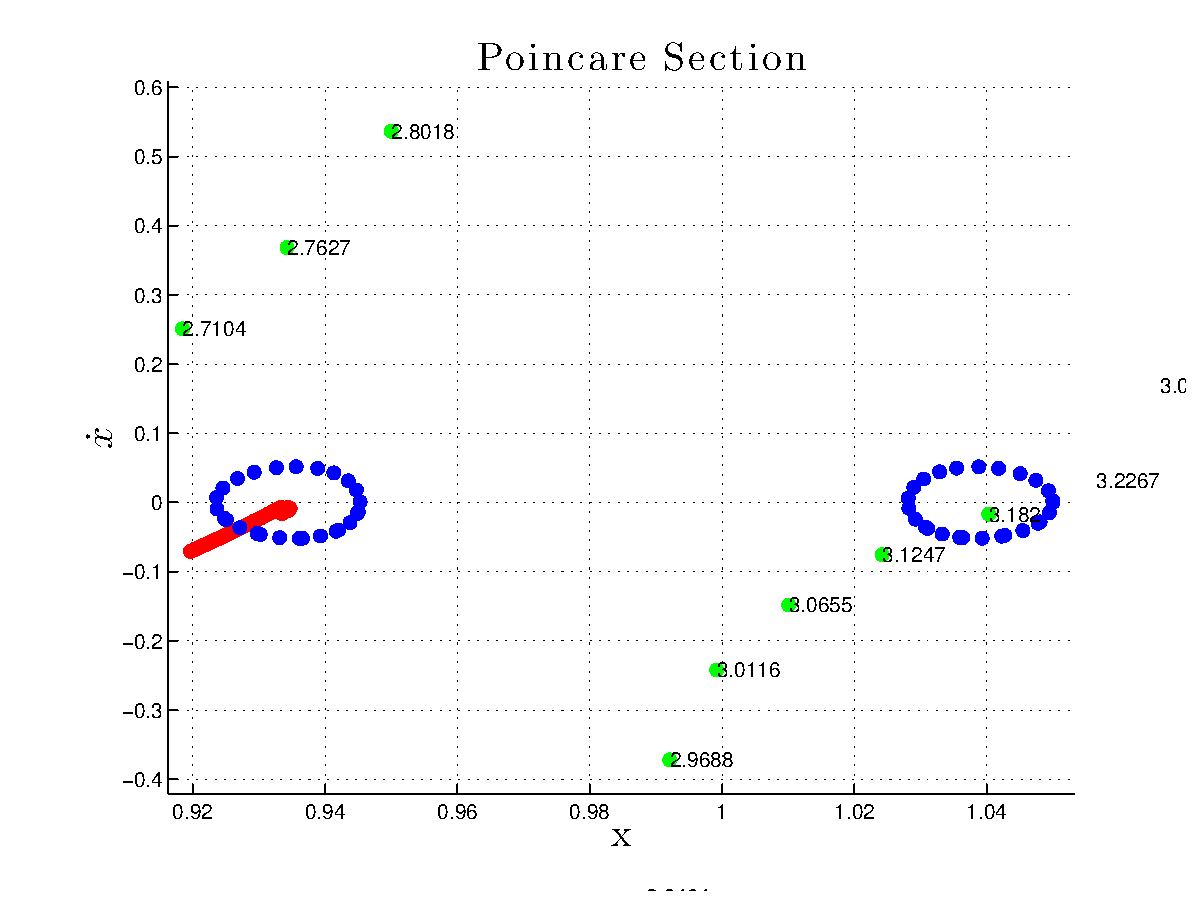
\includegraphics[width=\textwidth]{poincare_compare} 
	\end{subfigure} 
	\end{figure}

\end{frame} %--------------------------------------------------%